\documentclass[aspectratio=169]{beamer}
\usetheme{Madrid}
\usecolortheme{beaver}

% Packages
\usepackage{graphicx}
\usepackage{tikz}
\usepackage{pgfplots}
\usepackage{fontawesome5}
\usepackage{multicol}

% Title page information
\title[ARPMP]{Academic Research and Project Management Platform}
\subtitle{Revolutionizing Academic Research and Project Collaboration}
\author{Team Name}
\institute{Yukti Innovation Challenge 2025}
% \date{\today}

% Custom colors
\definecolor{narmpblue}{RGB}{25, 118, 210}
\definecolor{narmporange}{RGB}{255, 152, 0}
\definecolor{narmpgreen}{RGB}{76, 175, 80}

\begin{document}

% Title slide
\begin{frame}
\titlepage
\begin{center}
\vspace{-0.5cm}
\textcolor{narmpblue}{\faGlobe} \textcolor{narmporange}{\faUsers} \textcolor{narmpgreen}{\faRocket}
\end{center}
\end{frame}

% Problem Statement
\begin{frame}{The Problem We're Solving}
\begin{columns}
\begin{column}{0.5\textwidth}
\textbf{Current Academic Research Challenges:}
\begin{itemize}
\item  \faEyeSlash\  students' \textcolor{red}{lack of exposure} to ongoing research and projects.
\item \faExclamationTriangle\ \textcolor{red}{ No collaboration} among researchers of different institutes.
\item \faTrash\ \textcolor{red}{No repository} of the current status of projects done by passing out students.


\item \faCopy\ Resource \textcolor{red}{duplication} without awareness
\item \faChartLine\ \textcolor{red}{Inconsistent} quality tracking
\item  No unified and centralized tracking of projects.
\item \faUsers\ \textcolor{red}{Limited} mentor-student collaboration tools
\end{itemize}
\end{column}
\begin{column}{0.5\textwidth}
\begin{center}
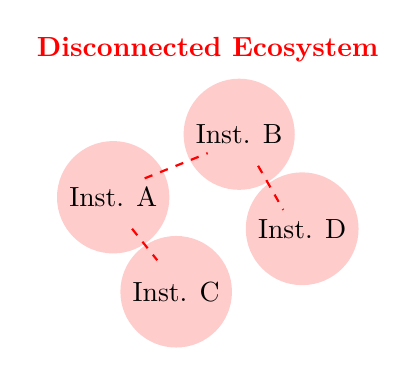
\begin{tikzpicture}[scale=0.8]
% Draw scattered institutions
\node[circle, fill=red!20, minimum size=1cm] at (0,0) {Inst. A};
\node[circle, fill=red!20, minimum size=1cm] at (2,1) {Inst. B};
\node[circle, fill=red!20, minimum size=1cm] at (1,-1.5) {Inst. C};
\node[circle, fill=red!20, minimum size=1cm] at (3,-0.5) {Inst. D};

% Draw disconnected arrows
\draw[thick, red, dashed] (0.5,0.3) -- (1.5,0.7);
\draw[thick, red, dashed] (0.3,-0.5) -- (0.7,-1);
\draw[thick, red, dashed] (2.3,0.5) -- (2.7,-0.2);

\node[above] at (1.5,2) {\textcolor{red}{\textbf{Disconnected Ecosystem}}};
\end{tikzpicture}
\end{center}
\end{column}
\end{columns}
\end{frame}

% Solution Overview
\begin{frame}{Our Solution: ARPMP}
\begin{center}
\textbf{\Large Academic Research and Project Management Platform}
\vspace{0.5cm}

\begin{tikzpicture}[scale=0.9]
% Central hub
\node[circle, fill=narmpblue!30, minimum size=2cm] at (0,0) {\textbf{ARPMP}};

% Connected levels
\node[rectangle, fill=narmpgreen!20, minimum width=2cm, minimum height=0.8cm] at (-3,2) {College Level};

\node[rectangle, fill=narmporange!20, minimum width=2cm, minimum height=0.8cm] at (3,2) {University Level};
\node[rectangle, fill=narmpblue!20, minimum width=2cm, minimum height=0.8cm] at (-3,-2) {Global Level};
\node[rectangle, fill=purple!20, minimum width=2cm, minimum height=0.8cm] at (3,-2) {National Level};

% Connecting arrows
\draw[thick, ->] (-0.8,0.8) -- (-1.5,1.3);
\draw[thick, ->] (0.8,0.8) -- (1.5,1.3);
\draw[thick, ->] (-0.8,-0.8) -- (-1.5,-1.3);
\draw[thick, ->] (0.8,-0.8) -- (1.5,-1.3);

% Features around
\node[ellipse, fill=yellow!20] at (0,3) {Mentorship};
\node[ellipse, fill=yellow!20] at (-4,0) {Collaboration};
\node[ellipse, fill=yellow!20] at (4,0) {Analytics};
\node[ellipse, fill=yellow!20] at (0,-3) {Knowledge Base};

\draw[dashed] (0,1.2) -- (0,2.5);
\draw[dashed] (-1.2,0) -- (-2.5,0);
\draw[dashed] (1.2,0) -- (2.5,0);
\draw[dashed] (0,-1.2) -- (0,-2.5);
\end{tikzpicture}
\end{center}
\end{frame}

% Solution Overview Slide
\begin{frame}{}

\vspace{0.5cm}

\begin{itemize}
\item ARPMP is a unified platform that digitizes and centralizes academic research and project management

\vspace{0.2cm}

\item Cloud-based multi-level platform (College → University → National → Global)

\vspace{0.2cm}

\item Mentor-student collaboration with progress tracking

\vspace{0.2cm}
\item Collaboration of multiple colleges on a project
\vspace{0.2cm}

\item Research archives, collaboration tools, resource libraries

\vspace{0.2cm}

\item Analytics for research trends, impact, and quality

\vspace{0.2cm}

\item AI-powered recommendations and mentorship matching

\end{itemize}

\end{frame}

% % Market Opportunity
% \begin{frame}{Market Opportunity}
% \begin{columns}
% \begin{column}{0.6\textwidth}
% \textbf{Target Market Size:}
% \begin{itemize}
% \item \faUniversity\ 50,000+ colleges in India alone
% \item \faUsers\ 40+ million students nationwide
% \item \faChalkboardTeacher\ 1.5+ million faculty members
% \item \faGlobe\ Global education technology market: \$350B+
% \end{itemize}

% \vspace{0.5cm}
% \textbf{Growth Drivers:}
% \begin{itemize}
% \item Digital transformation in education
% \item Government push for research excellence
% \item International collaboration requirements
% \item Quality assurance demands
% \end{itemize}
% \end{column}
% \begin{column}{0.4\textwidth}
% \begin{center}
% \begin{tikzpicture}
% \begin{axis}[
%     width=5cm,
%     height=4cm,
%     ybar,
%     xlabel=Years,
%     ylabel=Market Size (\$B),
%     symbolic x coords={2024,2026,2028,2030},
%     xtick=data,
%     ymin=0,
%     nodes near coords,
%     nodes near coords align={vertical},
% ]

% \addplot coordinates {
%     (2024,350)
%     (2026,420)
%     (2028,510)
%     (2030,625)
% };
% \end{axis}
% \end{tikzpicture}
% \end{center}
% \end{column}
% \end{columns}
% \end{frame}

% Target Users & Market
\begin{frame}{Target Users \& Market}

\begin{columns}[t]
\begin{column}{0.5\textwidth}
\textbf{User Types \& Value Provided:}
\vspace{0.3cm}

\begin{itemize}
\item \textbf{Students}
    \begin{itemize}
    \item Digital research profile
    \item Mentorship access
    \item Visibility
    \end{itemize}

\vspace{0.2cm}

\item \textbf{Mentors/Faculty}
    \begin{itemize}
    \item Dashboard to track students
    \item Feedback tools
    \item Analytics
    \end{itemize}

\vspace{0.2cm}

\item \textbf{Institutions (Colleges)}
    \begin{itemize}
    \item Archive research
    \item Generate reports
    \item Reduce duplication
    \end{itemize}
\end{itemize}
\end{column}

\begin{column}{0.5\textwidth}
\begin{itemize}
\item \textbf{Universities}
    \begin{itemize}
    \item Enable inter-college collaboration
    \item Manage funding
    \end{itemize}

\vspace{0.2cm}

\item \textbf{Government Agencies}
    \begin{itemize}
    \item National-level insights
    \item Policy alignment
    \end{itemize}

\vspace{0.2cm}

\item \textbf{Global Bodies}
    \begin{itemize}
    \item Cross-border research exchange
    \end{itemize}
\end{itemize}

\vspace{0.5cm}

\textbf{India Opportunity:}
\begin{itemize}
\item 50,000+ institutions
\item 38 million higher-ed students
\end{itemize}
\end{column}
\end{columns}

\end{frame}

% Key Features
\begin{frame}{Key Platform Features}
\begin{multicols}{2}
\textbf{\textcolor{narmpblue}{For Students:}}
\begin{itemize}
\item \faUser\ Personal research dashboard
\item \faArchive\ Access to senior projects
\item \faUsers\ Peer collaboration tools
\item \faChartLine\ Progress tracking
\item \faGraduationCap\ Skill development pathways
\end{itemize}

\textbf{\textcolor{narmporange}{For Mentors:}}
\begin{itemize}
\item \faTachometerAlt\ Comprehensive student management
\item \faChartBar\ Progress analytics
\item \faComments\ Integrated communication
\item \faShare\ Resource sharing
\item \faRobot\ AI-powered insights
\end{itemize}

\textbf{\textcolor{narmpgreen}{For Institutions:}}
\begin{itemize}
\item \faBuilding\ Multi-level coordination
\item \faHandshake\ Cross-institutional collaboration
\item \faFileAlt\ Automated reporting
\item \faDollarSign\ Funding management
\item \faAward\ Quality assurance
\end{itemize}

\textbf{\textcolor{purple}{For Administrators:}}
\begin{itemize}
\item \faGlobe\ National trend analysis
\item \faGavel\ Policy implementation
\item \faMoneyBill\ Funding distribution
\item \faNetworkWired\ Network facilitation
\item \faChartPie\ Impact assessment
\end{itemize}
\end{multicols}
\end{frame}

% Prototype of ARPMP - Slide 1: Landing Page Overview
\begin{frame}{Prototype of ARPMP}
\begin{center}
\textbf{\Large Landing Page - Platform Overview}
\end{center}

\vspace{0.5cm}

\begin{center}
% Replace with your actual image path
\includegraphics[width=0.9\textwidth,height=0.7\textheight,keepaspectratio]{Introduction.png}
\end{center}

\vspace{0.3cm}

\begin{center}
\textit{Comprehensive platform introduction showcasing multi-level research management}
\end{center}

\end{frame}

% Prototype of ARPMP - Slide 2: Landing Page Features
\begin{frame}{Prototype of ARPMP}
\begin{center}
\textbf{\Large Landing Page - Key Features}
\end{center}

\vspace{0.2cm}

\begin{center}
% Replace with your actual image path
\includegraphics[width=0.9\textwidth,height=0.7\textheight,keepaspectratio]{features.png}
\end{center}

\vspace{0.3cm}

\begin{center}
\textit{Platform capabilities and core functionalities demonstration}
\end{center}

\end{frame}

% Prototype of ARPMP - Slide 3: Landing Page Architecture
\begin{frame}{Prototype of ARPMP}
\begin{center}
\textbf{\Large Landing Page - System Architecture}
\end{center}

\vspace{0.2cm}

\begin{center}
% Replace with your actual image path
\includegraphics[width=0.9\textwidth,height=0.7\textheight,keepaspectratio]{levels.png}
\end{center}

\vspace{0.3cm}

\begin{center}
\textit{Multi-level integration from College to Global research networks}
\end{center}

\end{frame}

% Prototype of ARPMP - Slide 4: Mentor Dashboard
\begin{frame}{Prototype of ARPMP}
\begin{center}
\textbf{\Large Mentor Dashboard}
\end{center}

\vspace{0.2cm}

\begin{center}
% Replace with your actual image path
\includegraphics[width=0.9\textwidth,height=0.7\textheight,keepaspectratio]{mentor.png}
\end{center}

\vspace{0.3cm}

\begin{center}
\textit{Comprehensive mentor interface for student tracking and project management}
\end{center}

\end{frame}

% Prototype of ARPMP - Slide 5: Student Dashboard
\begin{frame}{Prototype of ARPMP}
\begin{center}
\textbf{\Large Student Dashboard}
\end{center}

\vspace{0.2cm}

\begin{center}
% Replace with your actual image path
\includegraphics[width=0.9\textwidth,height=0.7\textheight,keepaspectratio]{student.png}
\end{center}

\vspace{0.3cm}

\begin{center}
\textit{Student interface for research management and mentor collaboration}
\end{center}

\end{frame}

% Technology Stack
\begin{frame}{Technology & Architecture}
\begin{columns}
\begin{column}{0.5\textwidth}
\textbf{Frontend:}
\begin{itemize}
\item \faReact\ React.js + TypeScript
\item \faPalette\ Material-UI/Ant Design
\item \faChartBar\ Chart.js, D3.js
\item \faComments\ Socket.io (real-time)
\end{itemize}

\textbf{Backend:}
\begin{itemize}
\item \faNodeJs\ Node.js + Express.js
\item \faDatabase\ PostgreSQL + Redis
\item \faKey\ JWT + OAuth2
\item \faSearch\ Elasticsearch
\end{itemize}
\end{column}
\begin{column}{0.5\textwidth}
\textbf{Infrastructure:}
\begin{itemize}
\item \faCloud\ AWS/Google Cloud
\item \faDocker\ Docker + Kubernetes
\item \faShieldAlt\ Multi-layer security
\item \faChartLine\ Prometheus + Grafana
\end{itemize}

\textbf{AI/ML Features:}
\begin{itemize}
\item Recommendation engine
\item Collaboration matching
\item Trend prediction
\item Quality assessment
\end{itemize}
\end{column}
\end{columns}
\end{frame}


% Thank You
\begin{frame}
\begin{center}
{\Huge \textbf{Thank You}}

\vspace{1cm}
\textcolor{narmpblue}{\faHandsHelping} \textcolor{narmporange}{\faLightbulb} \textcolor{narmpgreen}{\faRocket}

\vspace{1cm}
\textbf{Let's Build the Future of Academic Research Together}
\end{center}
\end{frame}

\end{document}